\documentclass{article}
\usepackage{tikz}
\usetikzlibrary{shapes, shapes.multipart, arrows.meta, positioning, calc}

\begin{document}

\begin{figure}[htbp]
\centering
\resizebox{\textwidth}{!}{
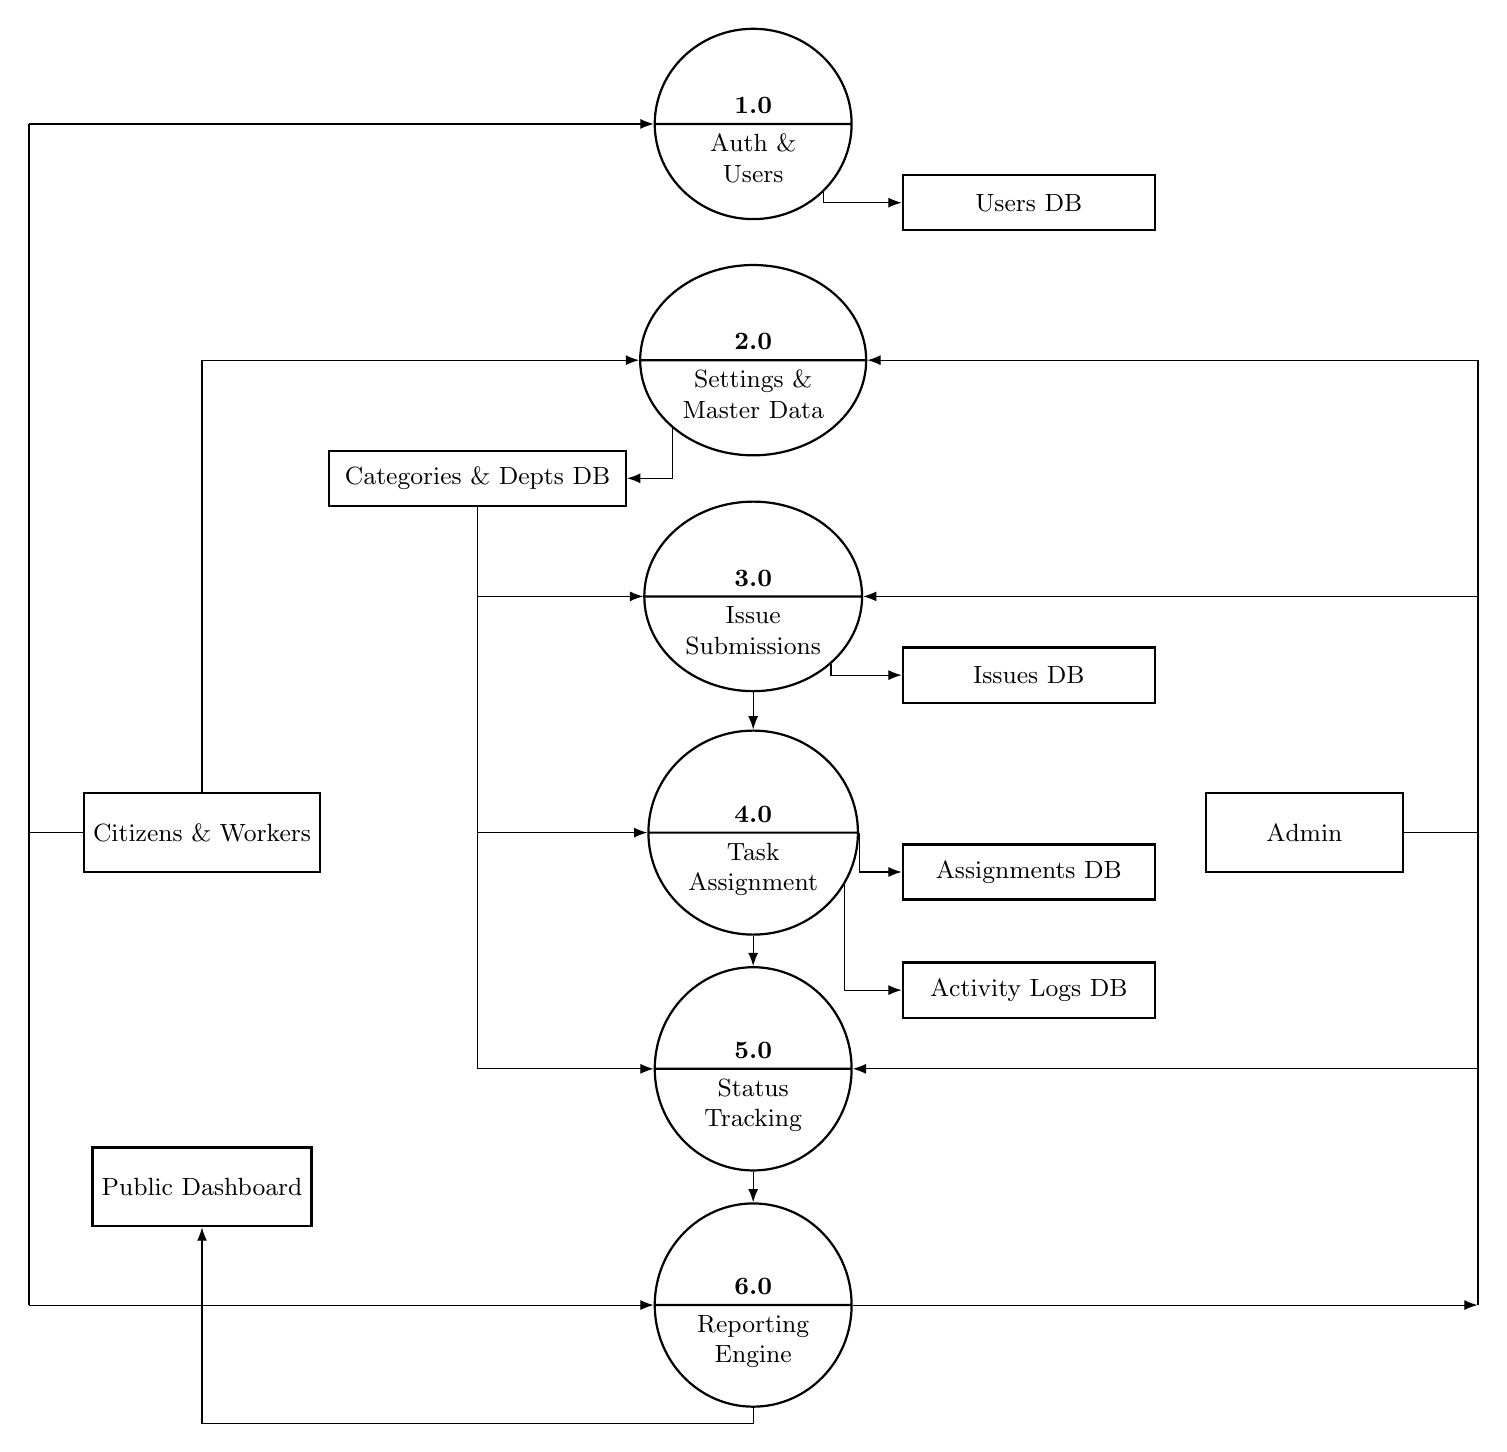
\begin{tikzpicture}[
    >=Latex,
    entity/.style={draw, rectangle, minimum width=2.5cm, minimum height=1cm, align=center, font=\small, fill=white, thick},
    process/.style={ellipse split, draw, minimum width=2.5cm, minimum height=1.5cm, align=center, font=\small, fill=white, thick},
    datastore/.style={
        draw, % <--- This instruction fully closes the rectangle!
        minimum width=3.2cm, minimum height=0.7cm, inner sep=0.2cm, font=\small, fill=white, thick,
        append after command={
            \pgfextra
                % Draws the inner vertical line on the left side
                \draw[thick] ([xshift=0.4cm]\tikzlastnode.north west) -- ([xshift=0.4cm]\tikzlastnode.south west);
            \endpgfextra
        }
    }
]

% -------------------------------------------------------------------------
% Exact Absolute Coordinates Grid Mapping to Guarantee Zero Overlaps!
% -------------------------------------------------------------------------

% Processes Column (x = 0)
\node[process] (P1) at (0, 0) { \textbf{1.0} \nodepart{lower} Auth \& \\ Users };
\node[process] (P2) at (0, -3) { \textbf{2.0} \nodepart{lower} Settings \& \\ Master Data };
\node[process] (P3) at (0, -6) { \textbf{3.0} \nodepart{lower} Issue \\ Submissions };
\node[process] (P4) at (0, -9) { \textbf{4.0} \nodepart{lower} Task \\ Assignment };
\node[process] (P5) at (0, -12) { \textbf{5.0} \nodepart{lower} Status \\ Tracking };
\node[process] (P6) at (0, -15) { \textbf{6.0} \nodepart{lower} Reporting \\ Engine };

% Left External Entities (x = -7)
\node[entity] (Adviser) at (-7, -9) {Citizens \& Workers};
\node[entity] (Viewer) at (-7, -13.5) {Public Dashboard};

% Right External Entities (x = 7)
\node[entity] (Admin) at (7, -9) {Admin};

% Left Data Stores (x = -3.5)
\node[datastore] (D2) at (-3.5, -4.5) {Categories \& Depts DB};

% Right Data Stores (x = 3.5)
\node[datastore] (D1) at (3.5, -1) {Users DB};
\node[datastore] (D3) at (3.5, -7) {Issues DB};
\node[datastore] (D4) at (3.5, -9.5) {Assignments DB};
\node[datastore] (D5) at (3.5, -11) {Activity Logs DB};

% -------------------------------------------------------------------------
% Structural Lines mapped using explicit coordinate joints
% -------------------------------------------------------------------------

% LEFT BUS (Adviser Backbone)
\draw[-, thick] (-9.2, 0) -- (-9.2, -15);
\draw[-] (Adviser.west) -- (-9.2, -9);
\draw[->] (-9.2, 0) -- (P1.west);
\draw[->] (-9.2, -15) -- (P6.west);

% Adviser specific hook to P2
% Neatly routes safely above the D2 Database!
\draw[->] (Adviser.north) |- (P2.west); 

% RIGHT BUS (Admin Backbone)
\draw[-, thick] (9.2, -3) -- (9.2, -15);
\draw[-] (Admin.east) -- (9.2, -9);
\draw[->] (9.2, -3) -- (P2.east);
\draw[->] (9.2, -6) -- (P3.east);
\draw[->] (9.2, -12) -- (P5.east);

% Reporting Engine pushing UP via the main Right Backbone Bus!
\draw[->] (P6.east) -- (9.2, -15); 

% LEFT DB (D2) Drop Bus 
% D2 connects from P2
\draw[->] (P2.south west) |- (D2.east);
% Drops vertically down x=-3.5 to cleanly miss all text and left entities
\draw[-] (D2.south) -- (-3.5, -12);
\draw[->] (-3.5, -6) -- (P3.west);
\draw[->] (-3.5, -9) -- (P4.west);
\draw[->] (-3.5, -12) -- (P5.west);

% Processes to RIGHT DBs
\draw[->] (P1.south east) |- (D1.west);
\draw[->] (P3.south east) |- (D3.west);
\draw[->] (P4.east) |- (D4.west);
\draw[->] (P4.330) |- (D5.west);

% Inter-Process straight links
\draw[->] (P3.south) -- (P4.north);
\draw[->] (P4.south) -- (P5.north);
\draw[->] (P5.south) -- (P6.north);

% P6 safely returning to Left Viewer (bottom loop)
\draw[->] (P6.south) -- (0, -16.5) -| (Viewer.south);

\end{tikzpicture}
}
\caption{1st Level Data Flow Diagram for Smart City Issue Reporting System}
\end{figure}

\end{document}
